\documentclass[tikz,border=12pt]{standalone}
\usepackage[T1]{fontenc}
\usepackage{mathpazo}
\usepackage{amsmath,amssymb}
\usetikzlibrary{arrows.meta, calc}

\definecolor{stblue}{HTML}{7B97AD}
\definecolor{rwgold}{HTML}{B8995E}
\definecolor{sage}{HTML}{7A9A7E}
\definecolor{dkbrown}{HTML}{3D3530}
\definecolor{wmgray}{HTML}{7B7067}
\definecolor{cream}{HTML}{F9F6F0}
\definecolor{border}{HTML}{D4C9B8}
\definecolor{terracotta}{HTML}{C47A6A}
\definecolor{lavender}{HTML}{907EA0}

\begin{document}
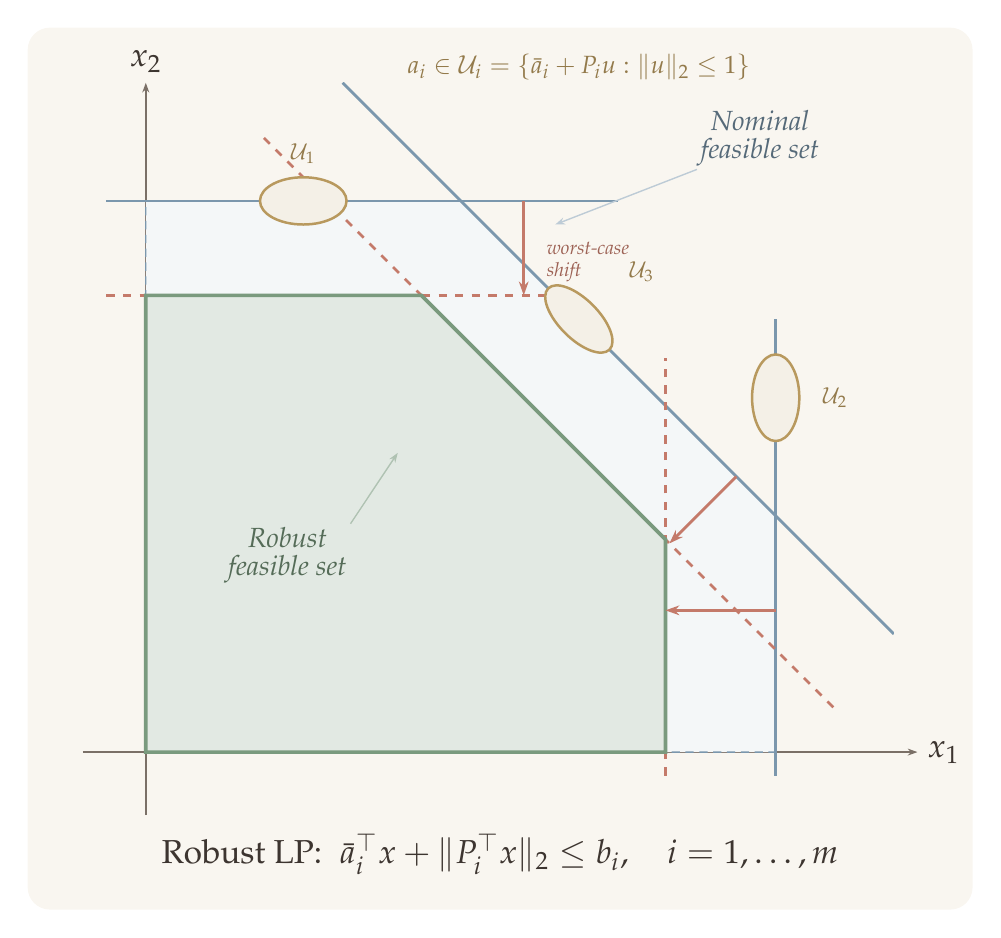
\begin{tikzpicture}[
    >={Stealth[length=3.5pt, width=2.5pt]},
    every node/.style={text=dkbrown},
  ]

  % Background
  \fill[cream, rounded corners=8pt] (-1.5,-2.0) rectangle (10.5,9.2);

  % === Axes ===
  \draw[->, wmgray, line width=0.8pt] (-0.8,0) -- (9.8,0)
    node[right, font=\large] {$x_1$};
  \draw[->, wmgray, line width=0.8pt] (0,-0.8) -- (0,8.5)
    node[above, font=\large] {$x_2$};

  % =========================================================
  % Three constraints (plus x1, x2 >= 0):
  %   C1: x2 <= 7               (horizontal upper)
  %   C2: x1 <= 8               (vertical right)
  %   C3: x1 + x2 <= 11         (diagonal, slope = -1)
  %
  % Nominal vertices:
  %   (0,0), (8,0), (8,3), (4,7), (0,7)
  %
  % Robust constraints (shifted inward):
  %   C1r: x2 <= 5.8
  %   C2r: x1 <= 6.6
  %   C3r: x1 + x2 <= 9.3
  %
  % Robust vertices:
  %   (0,0), (6.6,0), (6.6,2.7), (3.5,5.8), (0,5.8)
  % =========================================================

  % --- Nominal feasible region (light fill) ---
  \fill[stblue!8]
    (0,0) -- (8,0) -- (8,3) -- (4,7) -- (0,7) -- cycle;
  \draw[stblue, line width=0.5pt, densely dashed]
    (0,0) -- (8,0) -- (8,3) -- (4,7) -- (0,7) -- cycle;

  % --- Nominal constraint lines (stblue, solid) ---
  % C1: x2 = 7 — extend from left past the C3 intersection
  \draw[stblue, line width=1pt] (-0.5,7) -- (6.0,7);
  % C2: x1 = 8 — extend from bottom past the C3 intersection
  \draw[stblue, line width=1pt] (8,-0.3) -- (8,5.5);
  % C3: x1 + x2 = 11 — clip to a reasonable range
  \begin{scope}
    \clip (-0.5,-0.5) rectangle (9.5,8.5);
    \draw[stblue, line width=1pt] (2.5,8.5) -- (9.5,1.5);
  \end{scope}

  % --- Robust constraint lines (terracotta, dashed) ---
  % C1r: x2 = 5.8
  \draw[terracotta, line width=1pt, dashed] (-0.5,5.8) -- (5.5,5.8);
  % C2r: x1 = 6.6
  \draw[terracotta, line width=1pt, dashed] (6.6,-0.3) -- (6.6,5.0);
  % C3r: x1 + x2 = 9.3
  \begin{scope}
    \clip (-0.5,-0.5) rectangle (9.5,8.5);
    \draw[terracotta, line width=1pt, dashed] (1.5,7.8) -- (8.8,0.5);
  \end{scope}

  % --- Robust feasible region (sage, solid) ---
  \fill[sage!22]
    (0,0) -- (6.6,0) -- (6.6,2.7) -- (3.5,5.8) -- (0,5.8) -- cycle;
  \draw[sage, line width=1.3pt]
    (0,0) -- (6.6,0) -- (6.6,2.7) -- (3.5,5.8) -- (0,5.8) -- cycle;

  % === Uncertainty ellipses ON nominal constraint lines ===

  % U1 on C1 (x2=7, horizontal) at x1=2.0
  \fill[rwgold!15] (2.0,7.0) ellipse (0.55 and 0.30);
  \draw[rwgold, line width=0.9pt] (2.0,7.0) ellipse (0.55 and 0.30);
  \node[font=\footnotesize, rwgold!80!black] at (2.0,7.6) {$\mathcal{U}_1$};

  % U2 on C2 (x1=8, vertical) at x2=4.5
  \fill[rwgold!15] (8.0,4.5) ellipse (0.30 and 0.55);
  \draw[rwgold, line width=0.9pt] (8.0,4.5) ellipse (0.30 and 0.55);
  \node[font=\footnotesize, rwgold!80!black, right=5pt] at (8.3,4.5) {$\mathcal{U}_2$};

  % U3 on C3 (x1+x2=11, slope=-1, angle=-45deg)
  % Point on line: x1=5.5, x2=5.5. Check: 5.5+5.5=11.
  % Between the two vertices (4,7) and (8,3), on the boundary
  \fill[rwgold!15, rotate around={-45:(5.5,5.5)}]
    (5.5,5.5) ellipse (0.55 and 0.25);
  \draw[rwgold, line width=0.9pt, rotate around={-45:(5.5,5.5)}]
    (5.5,5.5) ellipse (0.55 and 0.25);
  \node[font=\footnotesize, rwgold!80!black] at (6.3,6.1) {$\mathcal{U}_3$};

  % === Shift arrows (nominal -> robust, perpendicular) ===

  % C1 shift: downward at x1=4.5
  \draw[-{Stealth[length=5pt, width=3.5pt]}, terracotta, line width=1pt]
    (4.8,7.0) -- (4.8,5.8);

  % C2 shift: leftward at x2=1.8
  \draw[-{Stealth[length=5pt, width=3.5pt]}, terracotta, line width=1pt]
    (8.0,1.8) -- (6.6,1.8);

  % C3 shift: perpendicular inward
  %   Perp distance = (11-9.3)/sqrt(2) = 1.2
  %   Start on C3 at (7.5, 3.5). Check: 7.5+3.5=11.
  %   End: (7.5-0.85, 3.5-0.85) = (6.65, 2.65)
  \draw[-{Stealth[length=5pt, width=3.5pt]}, terracotta, line width=1pt]
    (7.5,3.5) -- (6.65,2.65);

  % === Labels ===

  % "Nominal feasible set"
  \node[font=\normalsize, stblue!70!black, align=center]
    at (7.8,7.8) {\textit{Nominal}\\[-2pt] \textit{feasible set}};
  \draw[-{Stealth[length=3.5pt, width=2.5pt]}, stblue!50, line width=0.5pt]
    (7.0,7.4) -- (5.2,6.7);

  % "Robust feasible set"
  \node[font=\normalsize, sage!70!black, align=center]
    at (1.8,2.5) {\textit{Robust}\\[-2pt] \textit{feasible set}};
  \draw[-{Stealth[length=3.5pt, width=2.5pt]}, sage!60, line width=0.5pt]
    (2.6,2.9) -- (3.2,3.8);

  % "worst-case shift" annotation near C1 shift arrow
  \node[font=\scriptsize\itshape, terracotta!80!black, right=2pt]
    at (4.9,6.4) {worst-case};
  \node[font=\scriptsize\itshape, terracotta!80!black, right=2pt]
    at (4.9,6.1) {shift};

  % Ellipsoidal uncertainty formula
  \node[font=\small, rwgold!80!black]
    at (5.5,8.7) {$a_i \in \mathcal{U}_i = \{\bar{a}_i + P_i u : \|u\|_2 \leq 1\}$};

  % Bottom equation: the robust counterpart
  \node[font=\large, text=dkbrown, align=center] at (4.5,-1.3)
    {Robust LP: $\;\bar{a}_i^\top x + \|P_i^\top x\|_2 \leq b_i,
      \quad i=1,\ldots,m$};

\end{tikzpicture}
\end{document}
